\section{Problem 2}

problem 2

\subsection{Part1}


\begin{figure}[!htb]
\minipage{0.24\textwidth}
  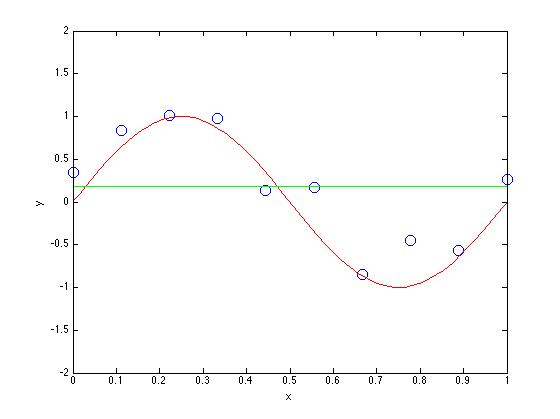
\includegraphics[width=\linewidth]{figures/p2_MLE_M=0}
  \caption{M = 0}\label{fig:figures/p2_MLE_M=0}
\endminipage\hfill
\minipage{0.24\textwidth}
  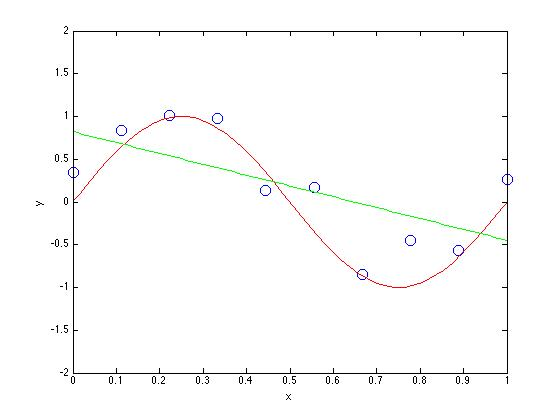
\includegraphics[width=\linewidth]{figures/p2_MLE_M=1}
  \caption{M = 1}\label{fig:figures/p2_M=1}
\endminipage\hfill
\minipage{0.24\textwidth}                                                                            
  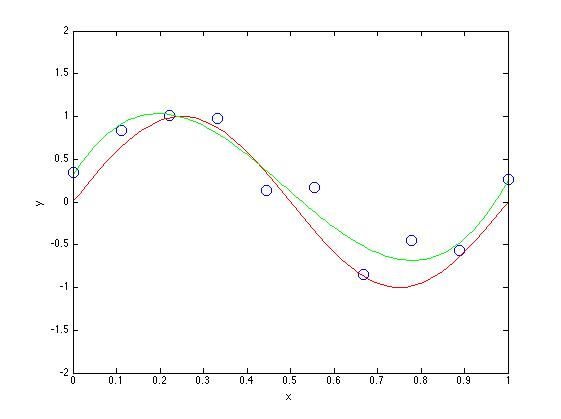
\includegraphics[width=\linewidth]{figures/p2_MLE_M=3}
  \caption{M = 3}\label{fig:figures/p2_M=3}
\endminipage\hfill
\minipage{0.24\textwidth}                                                                            
  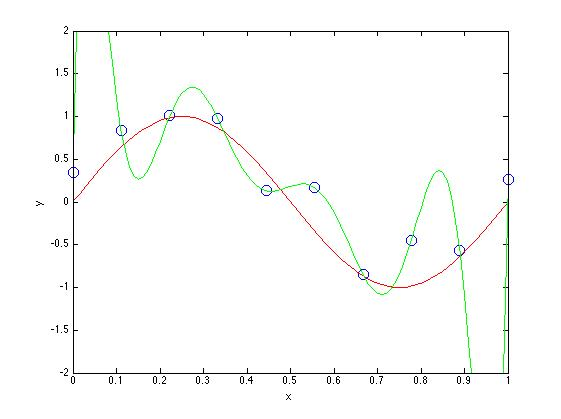
\includegraphics[width=\linewidth]{figures/p2_MLE_M=9}
  \caption{M = 9}\label{fig:figures/p2_M=9}
\endminipage\hfill
\end{figure}

we first computed the maximum likelihood weight vector and replicated 
the Bishop Figure 1.4. (The color is diffrent to show that it is generated). 



\subsection{Part2}

We tested a few data points using numerical gradient and analytical gradient for each function.
The error we observed is small for smaller Ms as explained in part 3 of problem 1. 

\subsection{Part3}

\begin{figure}[!htb]
\minipage{0.24\textwidth}
  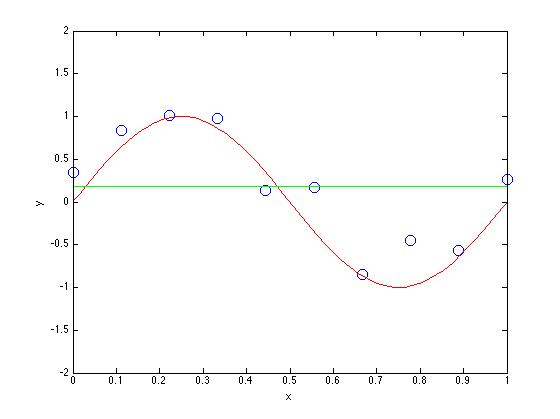
\includegraphics[width=\linewidth]{figures/p2_M=0}
  \caption{M = 0}\label{fig:figures/p2_M=0}
\endminipage\hfill
\minipage{0.24\textwidth}
  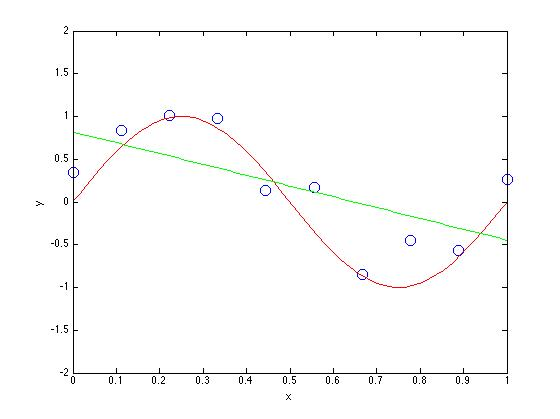
\includegraphics[width=\linewidth]{figures/p2_M=1}
  \caption{M = 1}\label{fig:figures/p2_M=1}
\endminipage\hfill
\minipage{0.24\textwidth}                                                                            
  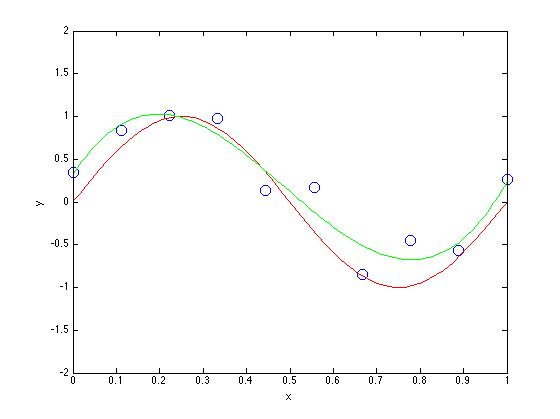
\includegraphics[width=\linewidth]{figures/p2_M=3}
  \caption{M = 3}\label{fig:figures/p2_M=3}
\endminipage\hfill
\minipage{0.24\textwidth}                                                                            
  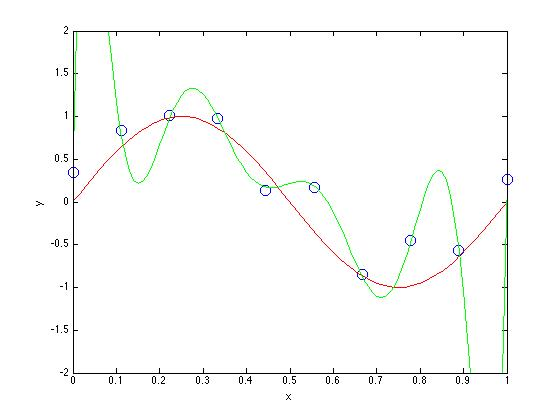
\includegraphics[width=\linewidth]{figures/p2_M=9}
  \caption{M = 9}\label{fig:figures/p2_M=9}
\endminipage\hfill
\end{figure}


we used gradient descent to replicate 
the Bishop Figure 1.4. (The color is diffrent to show that it is generated). 

